\documentclass{ltjsarticle}

\usepackage{amsmath}
\usepackage{amssymb}
\usepackage{amsthm}
\usepackage{ mathrsfs }
\usepackage{enumerate}
\usepackage{bbm}
\usepackage{lipsum}
\usepackage{fancyhdr}
\usepackage{tikz-cd} 
\usetikzlibrary{graphs}
\usepackage{luatexja-ruby} 
\usepackage{graphicx} 
\graphicspath{ {./images/} }

\newtheorem{theorem}{定理}[section] 
\newtheorem{proposition}{Proposition}[section] 
\newtheorem{definition}{定義}[section] 
\newtheorem{problem}{問題}
\newtheorem{postulate}{公準}[section] 
\newtheorem{lemma}{Lemma}[section] 
\newtheorem{notation}{Notation}[section] 
\newtheorem{remark}{注釈}[section] 
\newtheorem{corollary}{系}[section] 
\newtheorem{terminology}{Terminology}[section] 
\newtheorem{example}{例}[section] 
\newtheorem{step}{手順} 
\newtheorem{solution}{解答}[section] 
\newtheorem{fact}{事実}[section] 


\DeclareMathOperator{\diam}{diam}
\DeclareMathOperator{\Gal}{Gal}
\DeclareMathOperator{\rank}{rank}
\DeclareMathOperator{\Hom}{Hom}
\DeclareMathOperator{\Dom}{Dom}
\DeclareMathOperator{\Ann}{Ann}
\DeclareMathOperator{\grad}{grad}
\DeclareMathOperator{\Span}{Span}
\DeclareMathOperator{\interior}{int}
\DeclareMathOperator{\ind}{ind}
\DeclareMathOperator{\supp}{supp}
\DeclareMathOperator{\ob}{ob}
\DeclareMathOperator{\Spec}{Spec}
\DeclareMathOperator{\MaxSpec}{MaxSpec}
\DeclareMathOperator{\PreSh}{PreSh}
\DeclareMathOperator{\Sh}{Sh}
\DeclareMathOperator{\Fun}{Fun}
\DeclareMathOperator{\Ext}{Ext}
\DeclareMathOperator{\Aut}{Aut}
\DeclareMathOperator{\Ker}{Ker}
\DeclareMathOperator{\Image}{Im}
\DeclareMathOperator{\Coker}{Coker}
\DeclareMathOperator{\id}{id}
\DeclareMathOperator{\Mod}{Mod}
\DeclareMathOperator{\QCoh}{QCoh}
\DeclareMathOperator{\Coh}{Coh}
%\newcommand*{\name}[\num_arguments][default values]{{\color{#1}\Large #2}}
\newcommand*{\Z}{\mathbb{Z}}
\newcommand*{\Q}{\mathbb{Q}}
\newcommand*{\R}{\mathbb{R}}
\newcommand*{\multivar}[2]{{#1_1,\cdots,#1_{#2}}}
\newcommand*{\localization}[2]{#1_{\mathfrak{#2}}}
\newcommand*{\ringedspacemorph}[1]{(#1,#1^{\#})}
\newcommand*{\sheaf}[2]{(#1,{\mathcal{#2}}_{#1})}
\newcommand{\fib}[1]{%
  \mathbin{\mathop{\times}\limits_{#1}}%
}
\newcommand{\tens}[1]{%
  \mathbin{\mathop{\otimes}\displaylimits_{#1}}%
}
\title{授業ノート}
\author{ボン補習校高校数学}
\date{４月１８日}

\begin{document}

\maketitle

\section{極限の定義と微分}
人間の体はこの世界のことを知るには全く性能が足りません。この世界を作り出した知性がいるとするならば、人間の能力は憶えられる量も目で終える物体のスピードも、理解できる物事の種類も創造主に遠く及ばないでしょう。しかし、科学者たちは知恵を絞って我々が知れる、理解できる物事の数をどうやって増やせるのかを考えてきました。
\par 微分とは自然科学における顕微鏡です。生物の体は複雑ですが、顕微鏡で見ると小さなより単純な細胞の集まりだということがわかります。微分は数学における小さな細胞を調べるための道具を与えてくれます。数学における細胞とはズバリまっすぐな線です。人間の知能ではまっすぐなもの以外理解することが難しいですが、まっすぐな世界の知識を使ってどうやって曲がった世界のことを知れるのかを学んでいきます。
\subsection{集合}

\begin{definition}
集合とは数や図形、文字などをまとめて集りのことである。
\end{definition}

\begin{example}
整数全ての集合を$\Z$、有理数全ての集合を$\Q$、実数すべての集合を$\R$と書きます。
\end{example}

上の集合は全て無限の数の集まりですが、有限の数の集まりを考えることもあります。例えば$1$から$10$の数の集まりを
\begin{equation*}
\{1,2,3,4,5,6,7,8,9,10\}
\end{equation*}
というように書いたりします。またいくつかの数字を消したいとき。例えば$10$を消して$1$から$9$までの数の集まりを書くときは
\begin{equation*}
\{1,2,3,4,5,6,7,8,9\}=\{1,2,3,4,5,6,7,8,9,10\}\backslash\{10\}
\end{equation*}
というように書いたりします。
\begin{example}
$0$以外の整数全体の集合を$\Z\backslash\{0\}$と書いたりします。
\end{example}
\subsection{極限}
\begin{definition}
関数$f(x)$において、定義域とは$x$に代入できる全ての数の集合である。
\end{definition}

\begin{example}
次のような関数を考える。
\begin{equation*}
f(x) = {\frac {(x-1)(x+1)} {(x+1)}}
\end{equation*}
$x$に$-1$を代入すると。
\begin{equation*}
f(x) = {\frac {-2\times 0} {0}}
\end{equation*}
となり、$0$で割り算をしなくてはいけなくなります。よってこの関数の定義域は$-1$以外の全ての実数。よって
\begin{equation*}
\R\backslash\{-1\}
\end{equation*}
のようにかけます。
\end{example}

上の例では式を約分することにより関数を次のように表すことができます。
\begin{equation*}
f(x) = {\frac {(x-1)(x+1)} {(x+1)}}=(x-1)
\end{equation*}
数学では指定された書き方が重要なのでこの関数の定義域は$\R\backslash\{0\}$ですが、この形に注目すると$x=-1$の時の計算ができるようになります。このように最初の形では計算できないけれども、少し形を変えてあげることで計算できるようになる時、「本当はやってはいけないかもしれない」ということを強調するために
\begin{equation*}
\lim_{x\to-1}f(x) = \lim_{x\to-1}{\frac {(x-1)(x+1)} {(x+1)}} =\lim_{x\to-1}(x-1)= -2
\end{equation*}
というふうに書きます。

\begin{problem}
次の極限を計算せよ。
\begin{equation*}
\lim_{x\to 0} x, \quad\lim_{x\to 0} {\frac {x^2} x}, \quad\lim_{x\to 2} {\frac {(x-2)(x+2)}{x-2}}
\end{equation*}
\end{problem}

\subsection{$x^n$の微分}

最初に紹介した通り、まっすぐな世界を使って曲がった世界のことを調べることが微分のゴールです。二次関数を考えてみましょう。
\begin{center}
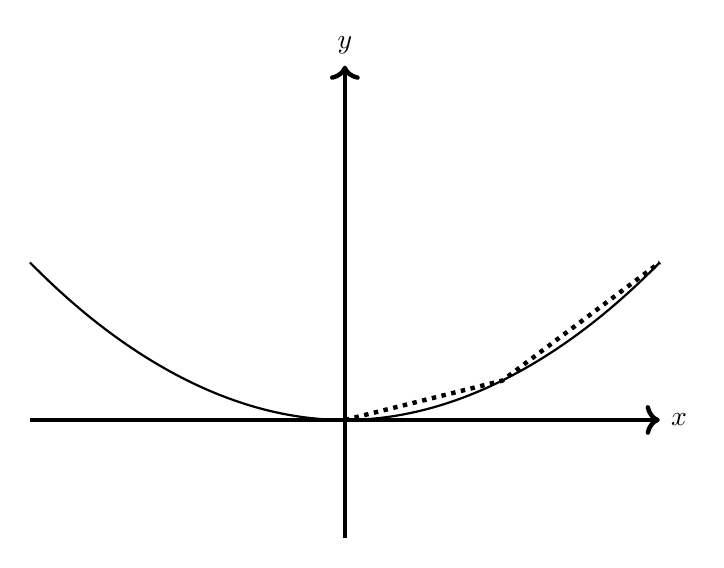
\begin{tikzpicture}
\draw[->,ultra thick] (-4,-1.5)--(4,-1.5) node[right]{$x$};
\draw[->,ultra thick] (0,-3)--(0,3) node[above]{$y$};
\draw[thick]  (0,-1.5) parabola (4,0.5);
\draw[thick] (0,-1.5) parabola (-4,0.5);
\draw[ultra thick, dotted] (0,-1.5) -- (2,-1)--(4,0.5);
\end{tikzpicture}
\end{center}

昔の人は曲がった図形は扱いにくいので、このように直線で形を似せることで計算を楽にしていました。しかし、正確にしようとすればするほど、線が折れている場所を増やす必要があり、どんどん難しくなっていきます。ここで発想を逆転させます。「調べたい部分が小さければ小さいほど、必要な折れた線の数は少なくなるのではないか。」ここで調べたい部分を限りなく小さくすることで、たった一つの直線で正確な計算をできるようにする。これが微分のアイデアです。
\par このアイデアは何も特別なものではなく、私たちは同じような現象を毎日見ています。地球は本当は丸いボールのような形ですが、私たちの見える世界はとても狭いので、小さな範囲では平らな世界に見えます。
\par 実際に計算してみましょう。下の図で$h$を限りなく小さくすると、

\begin{center}
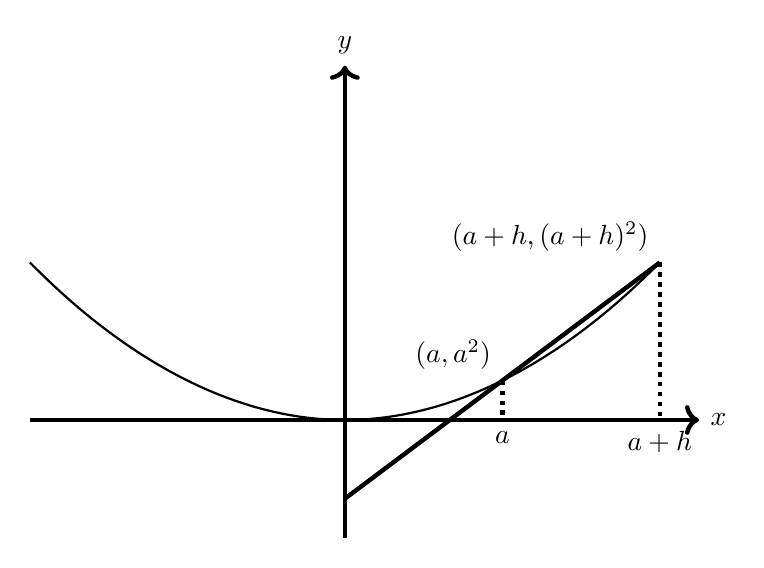
\begin{tikzpicture}
\draw[->,ultra thick] (-4,-1.5)--(4.5,-1.5) node[right]{$x$};
\draw[->,ultra thick] (0,-3)--(0,3) node[above]{$y$};
\draw[thick]  (0,-1.5) parabola (4,0.5);
\draw[thick] (0,-1.5) parabola (-4,0.5);
\draw[ultra thick] (0,-2.5) -- (4,0.5);
\draw[ultra thick, dotted] (2,-1)node[above left]{$(a,a^2)$}--(2,-1.5)[below]node{$a$};
\draw[ultra thick, dotted] (4,0.5)node[above left]{$(a+h,(a+h)^2)$}--(4,-1.5)[below]node{$a+h$};
\end{tikzpicture}
\end{center}
から
\begin{center}
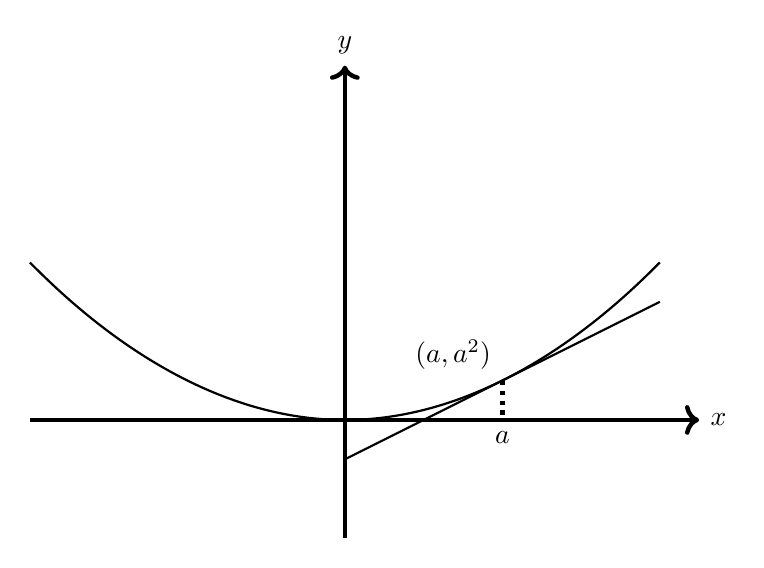
\begin{tikzpicture}
\draw[->,ultra thick] (-4,-1.5)--(4.5,-1.5) node[right]{$x$};
\draw[->,ultra thick] (0,-3)--(0,3) node[above]{$y$};
\draw[thick]  (0,-1.5) parabola (4,0.5);
\draw[thick] (0,-1.5) parabola (-4,0.5);
\draw[thick] (0,-2)--(2,-1) -- (4,0);
\draw[ultra thick, dotted] (2,-1)node[above left]{$(a,a^2)$}--(2,-1.5)[below]node{$a$};
\end{tikzpicture}
\end{center}
のように二次関数にピッタリとくっつく線が描けます。この直線は$(a,a^2)$を通ります。必要なのは傾きだけです。これを計算してみましょう。つぎの公式を使います。
\begin{equation*}
(a+b)^2 = a^2+2ab+b^2
\end{equation*}

これを使うと

\begin{align*}
(a+h)^2 = a^2+2ah+h^2
\end{align*}
よって最初の図において傾きは
\begin{equation*}
{\frac {(a+h)^2-a^2} {h}} 
\end{equation*}
$h$が限りなく小さくなると、
\begin{equation*}
\lim_{h\to0} {\frac {(a+h)^2-a^2} {h}} = \lim_{h\to0}{\frac {2ha+h^2} h} = \lim_{h\to0}2a+h = 2a
\end{equation*}
よってこの線は
\begin{equation*}
y - a^2 = 2a(x-a)
\end{equation*}
というように計算できます。このことをまとめましょう。
\begin{definition}
$f(x)$の$a$における微分とは
\begin{equation*}
{\frac {df} {dx}}(a) = \lim_{h\to0}{\frac {f(a+h)-f(a)} h}
\end{equation*}
である。
\end{definition}



\section{グラフとは}

\subsection{いろいろなグラフ}

グラフとは大まかにいうと、点とそれらをつなぐ線でてきた図のことです。例えば以下のような種類があります。
\begin{example}[単純グラフ]
もっともシンプルなグラフ。点とそれらをつなぐ線のみで作られている。 後に学びますが異なる点の間にある線は最大で一つのみかつ自分と自分をつなぐ線（ループ）が存在しないようなグラフのことを単純グラフと呼びます。
\begin{center}
\begin{figure}[h]
	\centering
    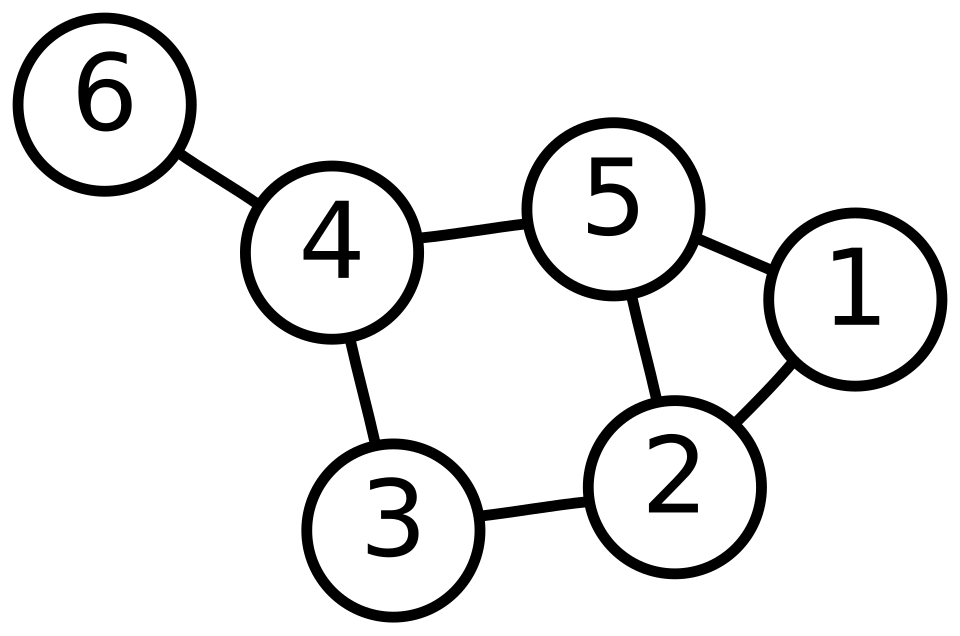
\includegraphics[scale=0.175]{graph}
    \caption{単純グラフ}
    \label{fig:simp_graph}
\end{figure}
\end{center}
\end{example}
\begin{example}[有向グラフ]
線に方向をつけたグラフ。道路などで一方通行の道や、電流、水の流れなど何か方向があるものを表すのに便利。
\begin{center}
\begin{figure}[h]
	\centering
    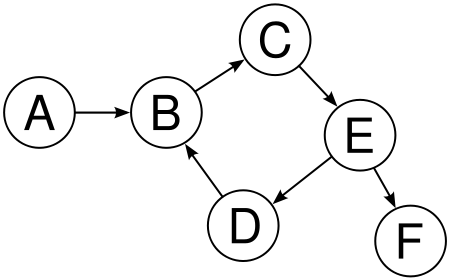
\includegraphics[scale=0.3]{directed_graph}
    \caption{有向グラフ}
    \label{fig:directed_graph}
\end{figure}
\end{center}
\end{example}
\begin{example}[重み付きグラフ]
点を街、線をそれらをつなぐ道路とした時に、移動にかかる時間の情報を線に追加して表すのに便利なグラフ。また流れる電気回路における電気抵抗を考える時などにも便利。
\begin{center}
\begin{figure}[h]
	\centering
    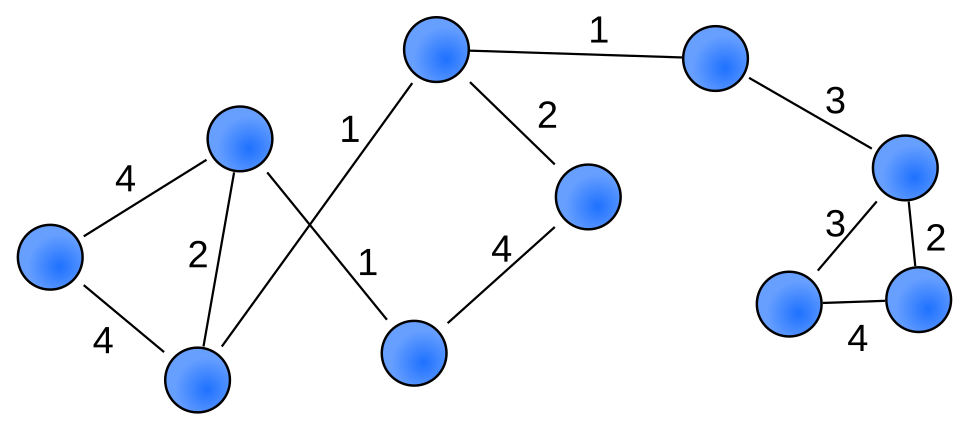
\includegraphics[scale=0.2]{weighted_graph}
    \caption{重み付きグラフ}
    \label{fig:weighted_graph}
\end{figure}
\end{center}
\end{example}

この授業では主に単純グラフのことを勉強します。

\subsection{単純グラフ}



\begin{definition}
グラフとは二つの集合のペア$(V,E)$で次の条件を満たすものである。
\begin{enumerate}[i).]
\item $V$を頂点の集合といい、$n$個の頂点があることを$V=\{1,2,3,\cdots,n\}$と書く。
\item $E$を辺の集合といい、二つの頂点$v,w\in V$をつなぐ辺があることを$\{v,w\}\in E$と書く。
\end{enumerate}
\end{definition}

この書き方を使って最初の単純グラフ
\begin{center}
\begin{figure}[h]
	\centering
    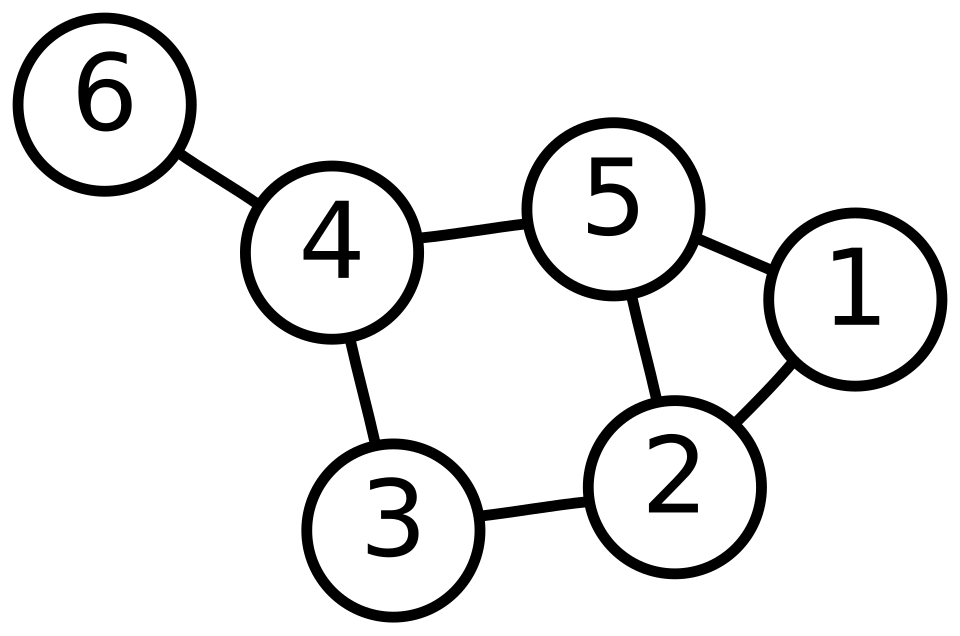
\includegraphics[scale=0.14]{graph}
    \caption{単純グラフ}
    \label{fig:simplegraph_example}
\end{figure}
\end{center}
を書いてみましょう。全部で$6$個の頂点があるので$V=\{1,\cdots,6\}$。辺は
\begin{equation*}
E=\{\{1,2\},\{1,5\},\{2,3\},\{2,5\},\{3,4\},\{4,5\},\{4,6\}\}
\end{equation*}
と書ける。

\begin{definition}
単純グラフとは、グラフのうち次の条件を満たすものである。
\begin{enumerate}[i).]
\item 二つの点の間には最大で一つの辺がある。
\item 自分自身を繋ぐ辺はない。
\end{enumerate}
\end{definition}

\begin{example}[単純グラフと非単純グラフ]\:
\begin{enumerate}
\item （左）は単純グラフ。
\item （真ん中）点の間に二つ以上の辺があるので単純グラフではない。
\item （右）自分自身を繋ぐ辺があるので単純グラフではない。
\end{enumerate}
\begin{center}
\begin{figure}[h]
	\centering
    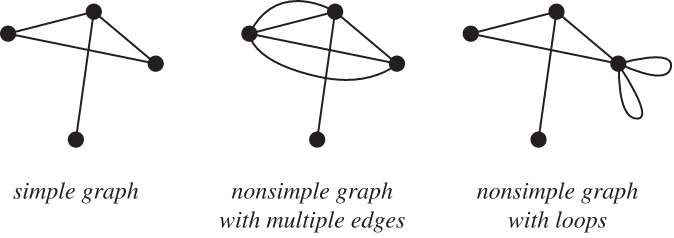
\includegraphics[scale=0.3]{simplegraph}
    \caption{単純グラフの例}
    \label{fig:simple_graph}
\end{figure}
\end{center}
\end{example}

単純グラフの中にも様々な形のグラフが存在します。

\begin{definition}
次のように始まりと終わりがあり、一直線に描けるグラフのことを道という。$n$この頂点を持つ道のことを$P_n$と書く。
\begin{center}
\begin{figure}[h]
	\centering
    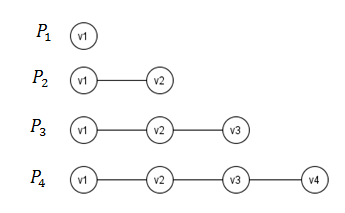
\includegraphics[scale=0.5]{paths}
    \caption{道の例}
    \label{fig:path}
\end{figure}
\end{center}
\end{definition}

\begin{definition}
次のように輪っかのように描けるグラフで辺を一つ取り除くと道になるグラフのことをサイクルという。$n$この頂点を持つサイクルのことを$C_n$と書く。
\begin{center}
\begin{figure}[h]
	\centering
    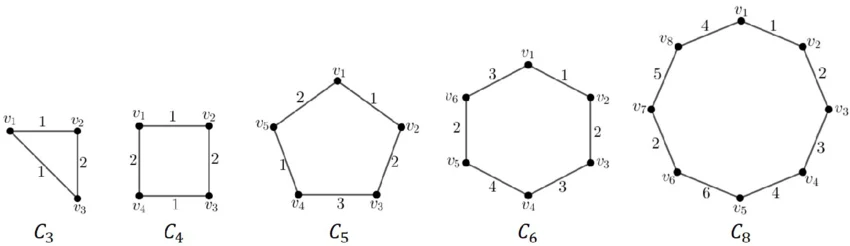
\includegraphics[scale=0.5]{cycles}
    \caption{閉路グラフの例}
    \label{fig:cycle}
\end{figure}
\end{center}\end{definition}
\:\\\\\\\\\\\:

\begin{definition}
次のように異なる二つの頂点の間に辺がちょうど一つあるグラフを完全グラフという。$n$この頂点を持つ完全グラフのことを$K_n$と書く。
\begin{center}
\begin{figure}[h]
	\centering
    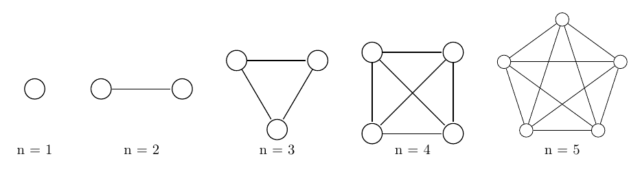
\includegraphics[scale=0.5]{complete_graphs}
    \caption{完全グラフの例}
    \label{fig:complete_graph}
\end{figure}
\end{center}\end{definition}

\begin{theorem}[握手の定理]
あるグラフにおいて、頂点の次数の和は辺の数の二倍。
\end{theorem}

\begin{proof}[証明]
グラフから辺を全て取り除いたグラフを考える。辺を一つずつ足していき元のグラフを作ることを考える。辺を一つ足すと次数の和は$2$増える。よって全ての辺を戻した時の次数の和は辺の数の二倍。
\end{proof}

\end{document}